\section{Software}
Ziel der Applikation ist es, die Berechnung der Schrittantwort eines Regelkreises zu visualisieren.\\
Die Applikation ist im Model-View-Controll Konzept aufgebaut. Die View erzeugt die Graphische Benutzeroberfläche. Dort können die spezifischen Werte zur Berechnung der Schrittantwort des Regelkreises eingegeben werden. Zudem wird diese Graphisch in einem Diagramm Festgehalten. Der Controller übernimmt die Steuerung der Applikation und übergibt die durchzuführenden Berechnungen an das Model weiter. Das Model führt alle Berechnungen zur Dimensionierung des Regelkreises durch, welche dann anschliessen in der View wieder visualisiert werden. Somit wäre der Kreislauf der Applikation geschlossen.\\
Zum Aufdatieren der Benutzerschnittstelle wird das Observable- Observer Entwurfsmuster verwendet. Die View agiert als Observer und das Model als Observable.


\subsection{Packages und seine Klassen}

\subsubsection{Package Controller}
Der Aufbau des Packages Controller ist in Abbildung \ref{packcontrl} ersichtlich.\\

\textbf{Controller}\\
Der Controller ist verantwortlich für die Steuerung der Applikation. Er stellt für alle Befehle die der Benutzer im GUI eine Methode zur Verfügung, mit der das Model modifiziert wird. Weiter erkennt er Fehleingaben und meldet diese dem Benutzer durch die Methode dispayError des Views. Bevor jeder Änderung des Models speichert sich der Controller eine Kopie des Modells, dadurch ist es möglich alte Zustände widerherzustellen und die Befehle Rückgängig und Wiederholen zu unterstützen. Weiter ist der Controller für das Speichern und Laden zuständig. Dies funktioniert da das Model das Serializable Interface implementiert und der Controller so die Daten mit einem ObjectOutputStream in eine Datei schreiben bzw. mit einem ObjectInputStream aus einer Datei laden kann. Der Controller ist nicht verantwortlich, dass das View die Daten des Models übernimmt, dies geschieht direkt durch die Klasse Observable (Observer Pattern).\\

\textbf{PIDRechner}\\
Startpunkt der Applikation. Initialisiert Controller, View und Model

\begin{figure}[p]
\centering
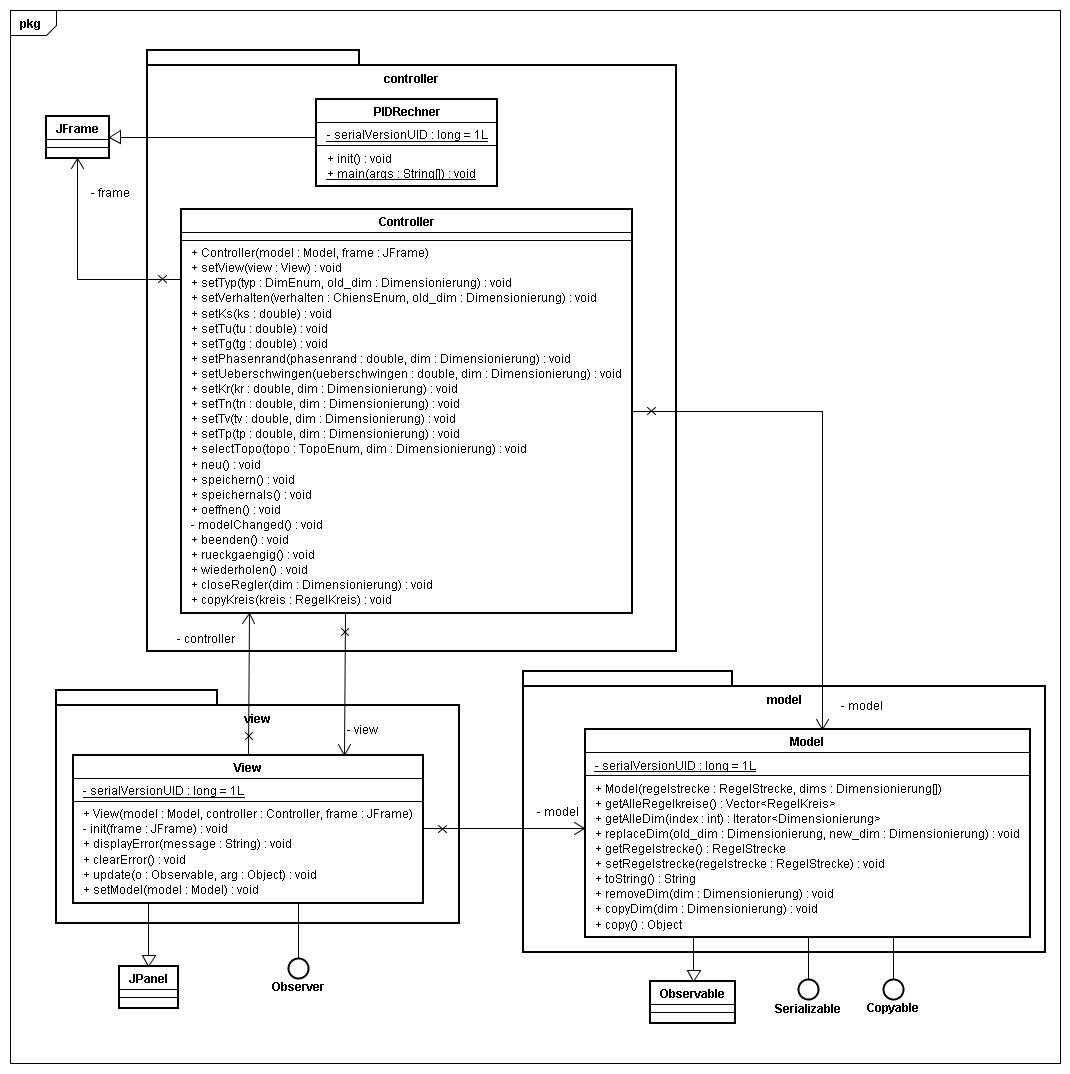
\includegraphics[width=1\textwidth]{packcontrl.png}
\caption{Package Controller}
\label{packcontrl}
\end{figure}

\newpage
\subsubsection{Package Model}
Der Aufbau des Packages Model ist in Abbildung \ref{packmodel} ersichtlich.\\

\textbf{Model}\\
Die Klasse Model verwaltet die Regelstecke und die verschiedenen Dimensionierungsmethoden. Es bietet Zugriffsmethoden um auf die Regelstrecke und Dimensionierungsmethoden zuzugreifen. Auch kann es Dimensionierungsmethoden kopieren oder löschen.\\

\textbf{Regelkreis}\\
Die Klasse Regelkreis dient zur Umwandlung der Übertragungsfunktionen von Regelstrecke und Regler in die Übertragungsfunktion des ganzen Kreises.\\

\textbf{Regelstrecke}\\
Die Klasse Regelstrecke bietet eine Abstraktion einer PTn-Strecke mit den Attributen Ks, Tu und Tg. Eine Regelstrecke ist ein Regelglied, das heisst sie kann als eine Übertragungsfunktion angesehen werden. Die Übertragungsfunktion wird durch die Sani-Approximation gebildet.\\

\textbf{Regler}\\
Diese Klasse dient zur Abstraktion eines PID-T Reglers mit den Parametern Kr, Tn, Tv, und Tp. Ein Regler wird normalerweise durch eine Dimensionierungsmethode gebildet.\\

\textbf{TransferFunction}
Eine Übertragungsfunktion besteht aus Zähler und Nenner. Sie bietet Methoden zur Faltung und Berechnung der Residuen. Weiter kann aus jeder Übertragungsfunktion eine Schrittantwort gebildet werden.\\

\textbf{Polynom}\\
Polynom abstrahiert reelle Polynome beliebigen Grades. Es bietet Methoden zur Addition und Multiplikation mit anderen Polynomen. Weiter können die Wurzeln und die Residuen (mit einem angenommenen Zähler von 1) ausgelesen werden.\\
 
\textbf{Schrittantwort}\\
Die Klasse Schrittantwort stellt die Schrittantwort für ein lineares Regelglied ohne Durchgriff dar. Sie bietet zudem Methoden zur Analyse. So kann sie feststellen ob eine Schrittantwort ausschwingt und wie gross An- und Ausschwingzeit sind. Weiter sucht sie nach dem Maximalwert der Kurve und bietet die Möglichkeit dessen Zeitpunkt und Grösse auszulesen.

\begin{figure}[p]
\centering
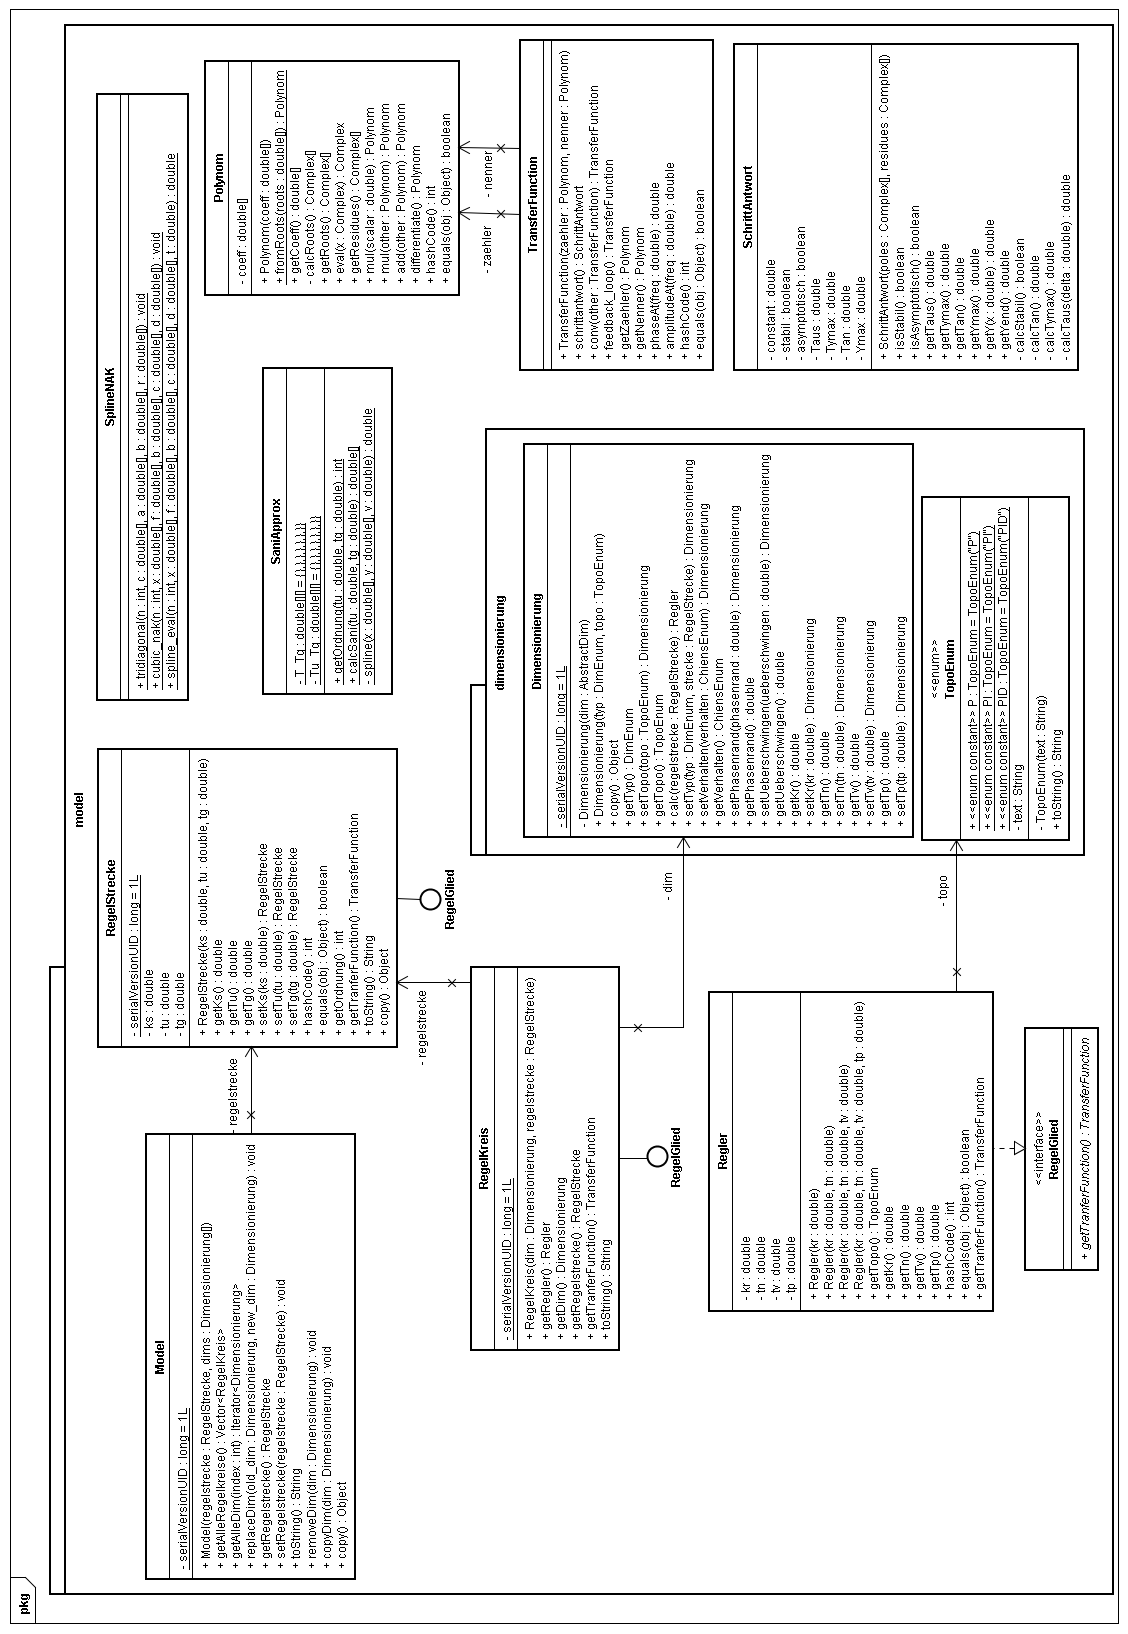
\includegraphics[width=1\textwidth]{packmodel.png}
\caption{Package Model}
\label{packmodel}
\end{figure}

\newpage
\subsubsection{Package Dimensionierung}
Der Aufbau des Packages Dimensionierung ist in Abbildung \ref{packdim} ersichtlich.\\

\textbf{Dimensionierung}\\
Diese Klasse ist ein tagged-Union der anderen Dimensionierungsarten. So bietet diese Klasse auch alle Methoden der anderen Dimensionierungsmethoden. Wird eine Methode bei einer falschen Variante verwendet, wirft die Klasse eine ClassCastException. Der Typ kann mit der Methode setTyp gewechselt werden. Beim Wechseln zu der Manuellen Dimensionierungsmethode, werden die Werte des dimensionierten Reglers übernommen.\\

\textbf{DimEnum}\\
Dieser Enum dient zur Aufzählung aller Dimensionierungstypen. Er ordnet jedem Typ auch einen Text zu.\\

\textbf{TopoEnum}\\
Zur Unterscheidung von PI und PID Reglern wird dieser Enum verwendet.\\

\textbf{AbstractDim}\\
AbstractDim ist die abstrakte Grundklasse aller Dimensionierungsmethoden. Die Methode calc berechnet für eine gegebene Regelstrecke einen Regler. Durch get- und setTopo lässt sich die Reglertopologie modifizieren. Die Methode getTyp() gibt den Typ des konkreten Reglers zurück.\\

\textbf{ZellwegerDim}\\
Hier steckt die Phasengangmethode zur Reglerdimensionierung. Die Beschreibung der Methode findet sich im theoretischen Teil.\\

\textbf{IterativDim}\\
Diese Methode führt die Phasengangmethode mehrmals nacheinander aus und sucht mit einer binären Suchmethode nach dem gewünschten Überschwingen der Schrittantwort.\\

Die anderen Klassen entsprechen den verschiedenen Faustregeln.

\begin{figure}[p]
\centering
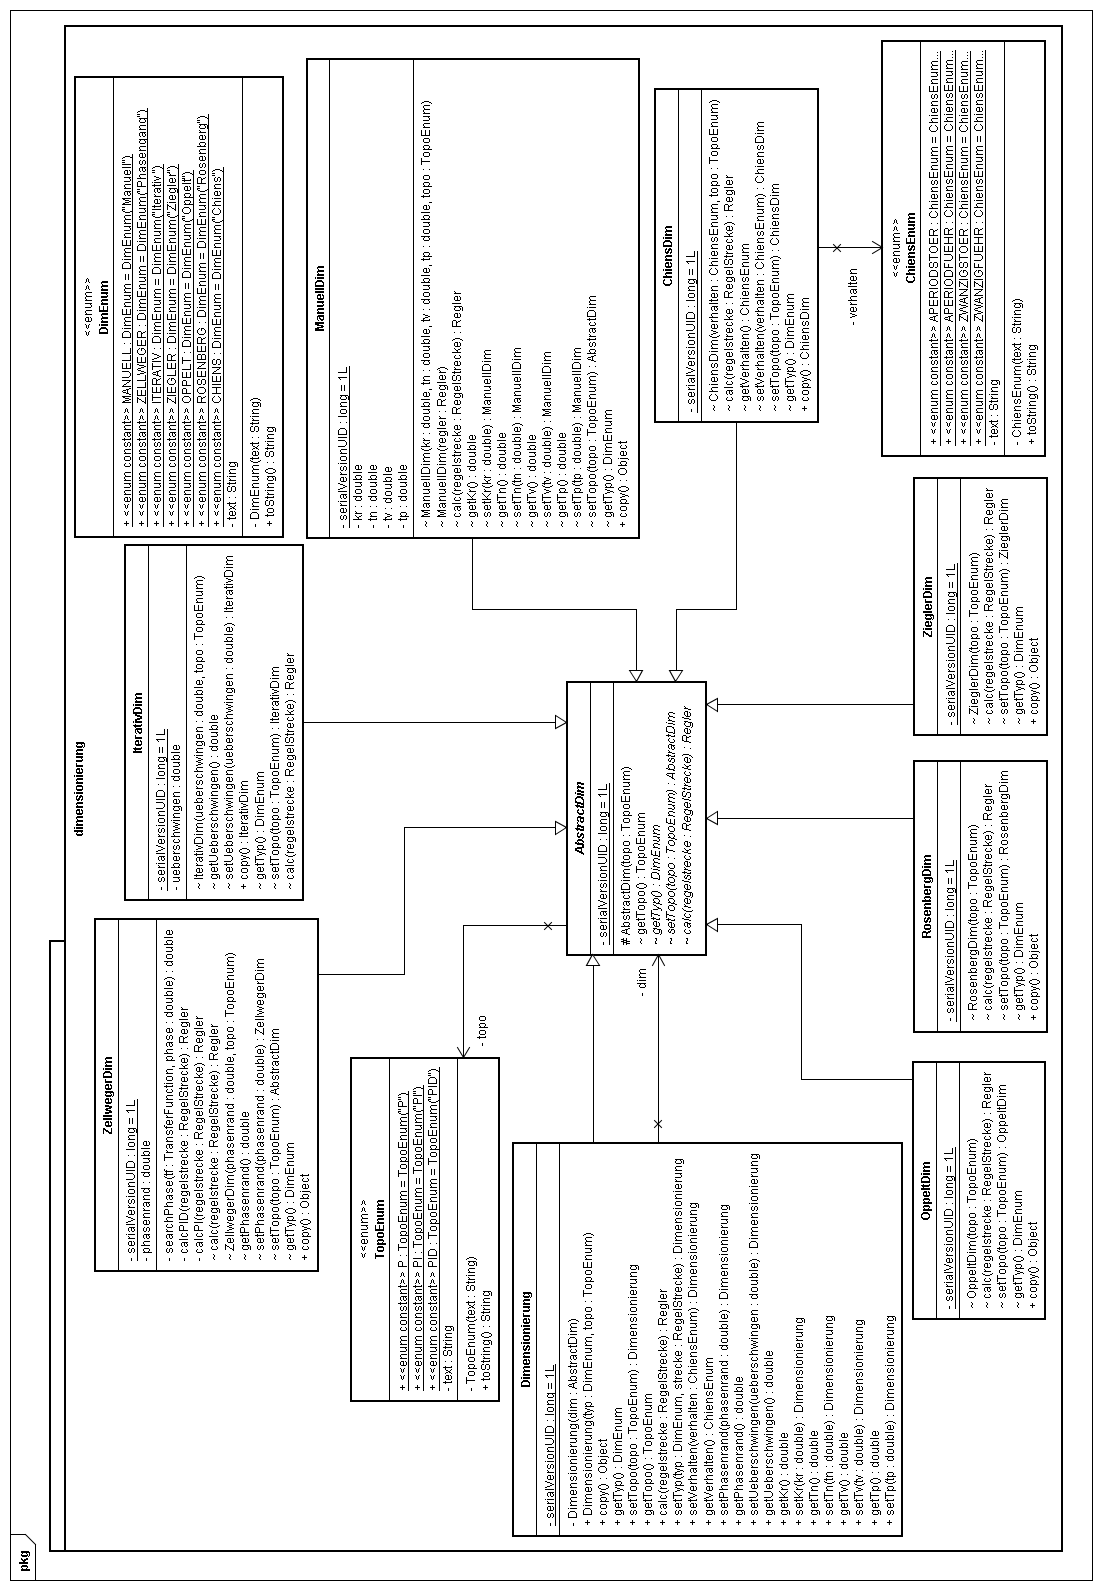
\includegraphics[width=1\textwidth]{packdim.png}
\caption{Package Dimensionierung}
\label{packdim}
\end{figure}

\newpage
\subsubsection{Package View}
Der Aufbau des Packages View ist in Abbildung \ref{packview} ersichtlich.\\

\textbf{View}\\
View ist die oberste Ebene im GUI (abgesehen vom Frame). Es beheimatet die Sidebar, den Graph und die Statuszeile. Auch initialisiert es die Menübar vom JFrame.\\

\textbf{SidebarPanel}\\
SidebarPanel ordnet die einzelnen Panels von Regelstrecke, Regler und Analyse vertikal untereinander an.\\

\textbf{RegelstreckeView}\\
RegelstreckeView zeigt die Parameter der Regelstrecke sowie die berechnete Ordnung und die Zeitkonstanten an.\\

\textbf{ReglerView}\\
Dieses JPanel visualisiert den Typ der Dimensionierungsmethode, deren Parameter und die Werte des daraus resultierenden Reglers.\\

\textbf{AnalyseView}\\
Zeigt die Eigenschaften einer Schrittantwort.\\

\textbf{Graph}\\
Zeichnet alle Schrittantworten mit dem ChartPanel von JFreeChart. Unter dem Graphen zeigt es weiter eine Legende. Die Zustände der Checkboxen werden nur vom Graph selbst verwendet und nicht dem Controller mitgeteilt.

\begin{figure}[p]
\centering
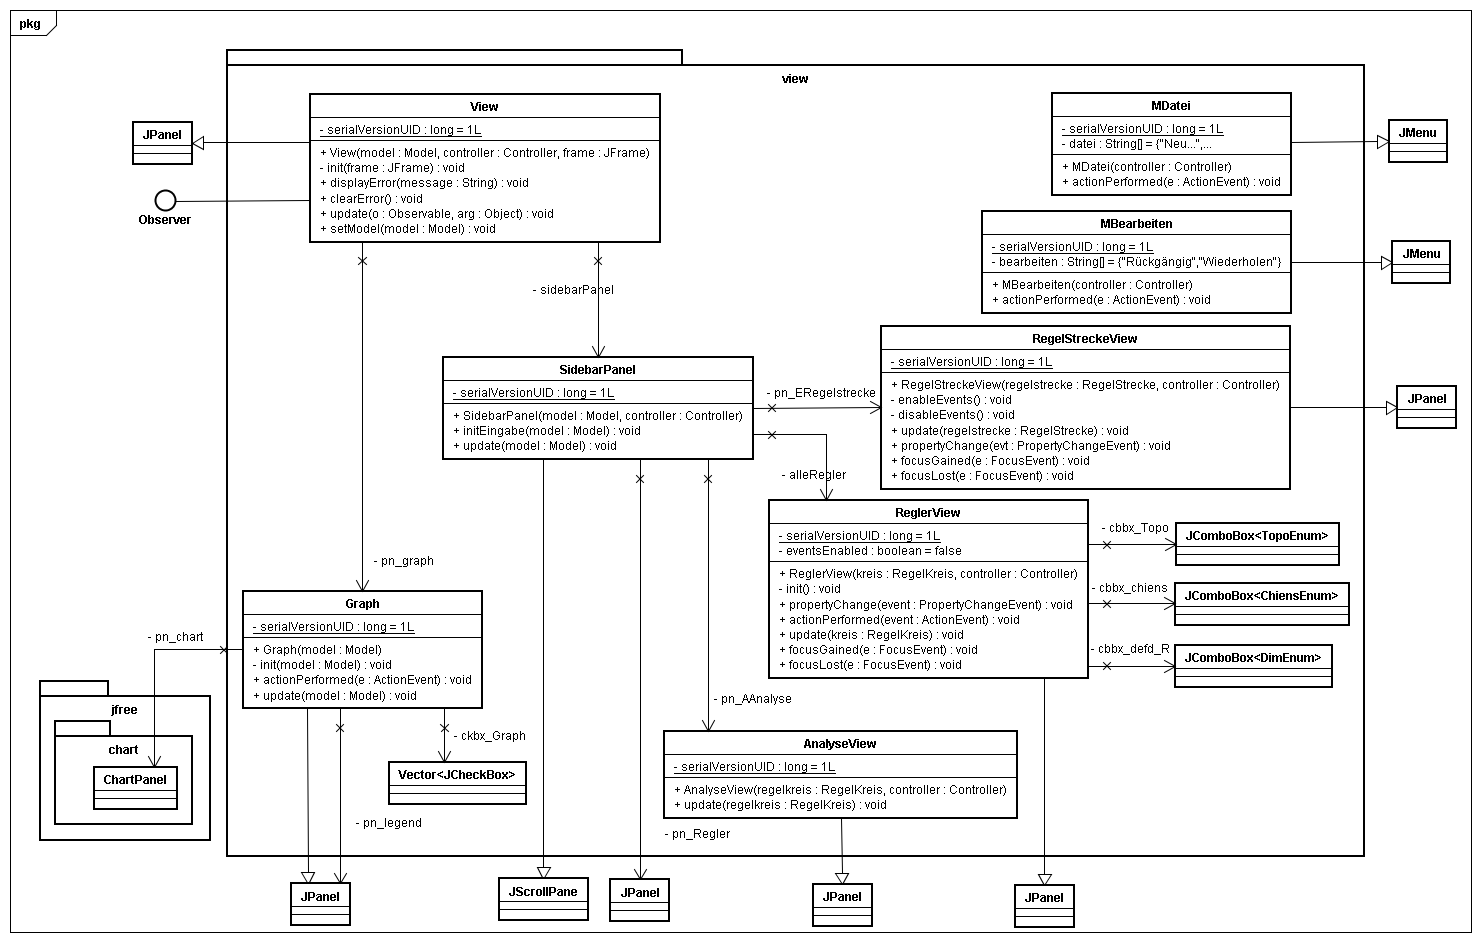
\includegraphics[width=0.9\textwidth]{packview.png}
\caption{Package View}
\label{packview}
\end{figure}
